% Chương 4 (sửa trực tiếp; bản tiếng Việt)
\chapter{ĐÁNH GIÁ VÀ QUYỀN RIÊNG TƯ}

\section{Thiết lập đánh giá}

Hệ thống được đánh giá ở bốn mức: độ bao phủ phát hiện, quyết định cho từng học sinh, ước lượng cấp lớp và hiệu năng trên thiết bị. Luận văn dùng nhiều nguồn bằng chứng, vì không có bộ dữ liệu đơn lẻ nào có nhãn sự chú ý theo từng học sinh cho các buổi giảng thực.

\textbf{Hệ thống được kiểm tra.} hcpose trên Raspberry Pi 5 với Hailo-8 AI HAT (26 TOPS), Raspberry Pi OS trixie, HailoRT 4.23 / TAPPAS 5.1. Các mô hình tư thế là mô hình YOLOv8-pose phần thân trên (13 điểm khóa) của chính dự án ở ba kích thước n, s và m, biên dịch thành HEF INT8. Trọng số mô hình được giữ cố định trong suốt quá trình: mọi cải tiến nằm ở tiền xử lý, hậu xử lý và logic đánh giá mức độ tập trung.

\textbf{Bằng chứng}

\begingroup\small
\begin{xltabular}{\textwidth}{*{4}{>{\raggedright\arraybackslash}X}}
\caption{Các nguồn bằng chứng dùng trong đánh giá}\label{tab:sources-of-evidence-used-in-the-evaluati}\\
\toprule
\textbf{Nguồn} & \textbf{Nội dung} & \textbf{Đo lường gì} & \textbf{Nhãn} \\
\midrule
\endfirsthead
\multicolumn{4}{l}{\emph{(tiếp theo)}}\\
\toprule
\textbf{Nguồn} & \textbf{Nội dung} & \textbf{Đo lường gì} & \textbf{Nhãn} \\
\midrule
\endhead
\bottomrule
\endlastfoot
SCB-Dataset (ba tập con) \cite{b3} & 8.116 ảnh lớp học duy nhất sau khi gộp ảnh trùng, phổ thông Trung Quốc & độ bao phủ phát hiện, độ chính xác bộ phân loại theo từng học sinh (kiểm định chéo 5 phần nhóm theo tiết học) & hộp hành động: đọc, viết, giơ tay (tập trung); TurnHead, BowHead, thảo luận (mất tập trung) \\
Video phòng thi \cite{b17} & 72 s, camera đặt cao ở góc, khoảng 30 học viên người lớn đang viết & báo động nhầm, ước lượng cấp lớp & không có; bối cảnh cho thấy tỷ lệ gần 0 \\
Video phòng tự học \cite{b18} & 6 phút, camera ngang mặt bàn, khoảng 50 học sinh & phòng đông, đếm chỗ ngồi, lỗi khi camera thấp & không có; bối cảnh cho thấy tỷ lệ thấp \\
Video buổi giảng \cite{b19} & 3 phút 18 s, camera đặt cao phía trước, khoảng 35 học sinh, phần lớn chăm chú & khả năng chuyển giao của các bộ phân loại sang buổi giảng thực & không có; bối cảnh cho thấy tỷ lệ gần 0 \\
Video lớp nhỏ (clip\_5) & 14 phút, iPhone gắn cao phía trước, 10 học sinh phổ thông ở ba hàng; một kịch bản sơ bộ mà học sinh không làm theo đều đặn & báo động nhầm và phát hiện đúng trên một lớp chưa từng dùng để tinh chỉnh; đếm chỗ ngồi ở khoảng cách gần & 150 thời điểm học sinh được gán nhãn mù \\
Buổi dàn dựng hai người (clip\_4) & 4 phút 45 s, điện thoại gắn cao phía trước, hai người lớn diễn 7 sự kiện theo kịch bản & recall, precision, độ trễ, báo động nhầm khi viết & chính xác theo từng giây, từ kịch bản \\
Nhãn do người gán & 301 thời điểm học sinh từ hai video, gán nhãn mù & precision và recall trên lớp học thực & tập trung / mất tập trung / không rõ \\
\end{xltabular}
\endgroup

\textbf{Độ đo.} Độ bao phủ = tỷ lệ học sinh có nhãn được ghép với một phát hiện (độ phủ tâm ≥ 0.5 hoặc IoU ≥ 0.3). Theo từng học sinh: AUC, AUC trong ảnh (chỉ các ảnh có cả hai lớp, loại bỏ lối tắt ``nhận ra bức ảnh''), balanced accuracy, precision và recall của lớp \emph{mất tập trung}. Cấp lớp: tỷ lệ mất tập trung trung bình của lớp, độ rộng khoảng 95\% của nó, và sĩ số suy ra. Thiết bị: FPS, độ trễ, CPU, bộ nhớ, nhiệt độ, giảm xung, công suất.

Số liệu trên SCB lấy từ HEF INT8 của m khi triển khai, trừ khi có ghi chú khác. Số liệu trên các video lấy từ các HEF INT8 trên Pi; hai biểu đồ và điểm số theo nhãn người gán dùng cùng mô hình n ở FP32 trên PC, và các lần chạy INT8 tái hiện kết quả này với sai khác vài điểm.

\section{Độ bao phủ phát hiện và chia ô ảnh}

Không có chia ô ảnh, mô hình bỏ sót phần lớn học sinh ở các hàng xa; chạy lại trên ba ô phóng to phủ 60\% phía trên của khung hình nâng độ bao phủ từ 48.6\% lên 75.5\% số học sinh có nhãn ở ngưỡng 0.3, và từ 17.0\% lên 74.4\% ở một phần ba xa nhất.

\begin{figure}[htbp]
\centering
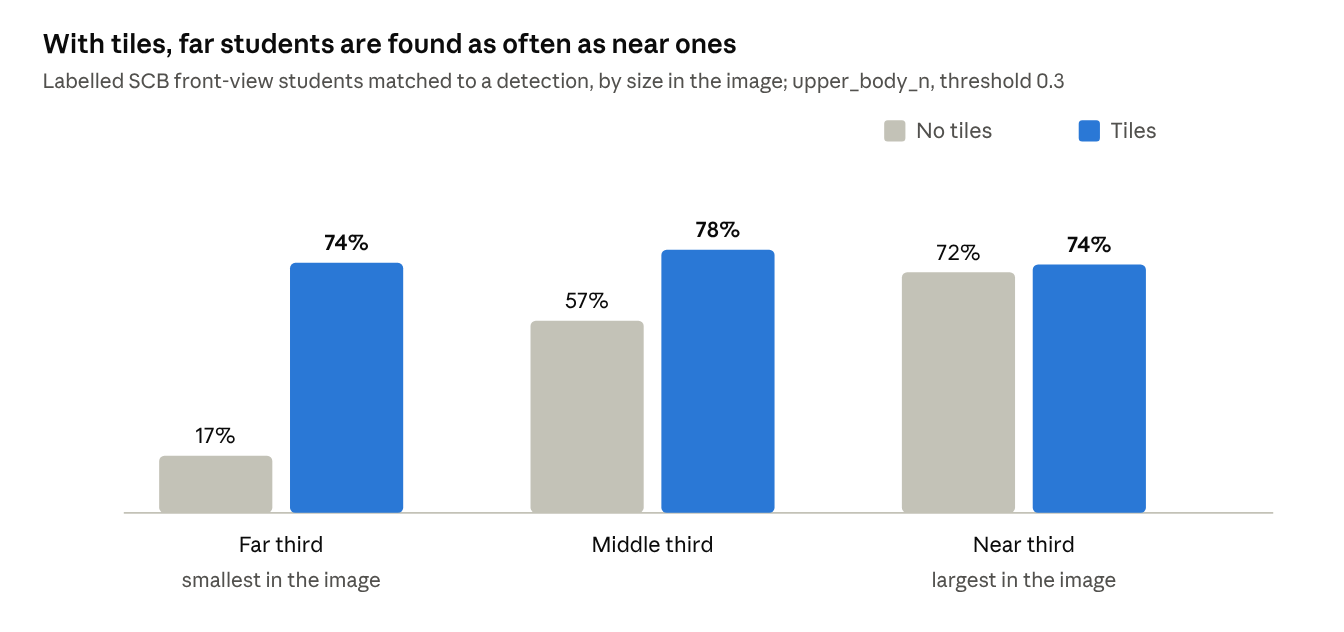
\includegraphics[width=0.8\textwidth]{figures/scb_coverage.png}
\caption{Học sinh nhìn chính diện có nhãn trong SCB được phát hiện, theo kích thước trong ảnh, khi không có và có chia ô (upper\_body\_n, ngưỡng 0.3)}\label{fig:labelled-scb-front-view-students-detecte}
\end{figure}

\textbf{Phương pháp.} Ngoài khung hình đầy đủ, mô hình chạy trên một hàng các ô gần vuông, chồng lấn nhau, phủ 60\% phía trên của ảnh (ba ô ở độ phân giải 1280×720). Phát hiện trong các ô được ánh xạ về khung hình; các phát hiện bị cắt bởi cạnh trong của ô bị loại, và các phát hiện trùng giữa các lượt được gộp theo IoU, hoặc theo quan hệ bao chứa kèm điểm khóa khớp nhau. Cả hai engine cài đặt cùng các luật này; kết quả gộp bằng C++ trong pipeline GStreamer được kiểm tra là trùng với kết quả gộp bằng Python trên 25 cảnh ngẫu nhiên. Trọng số bộ phát hiện không thay đổi.

\textbf{Trên mô hình m INT8 khi triển khai}, số học sinh nhìn chính diện trong SCB được ghép tăng từ 23.186 khi không chia ô lên 36.226 khi có chia ô (+56\%); 13.269 học sinh chỉ được tìm thấy khi có chia ô, 229 chỉ được tìm thấy khi không chia ô.

\textbf{Trên các video lớp học}, số học sinh mỗi khung hình:

\begin{table}[htbp]\small
\caption{Số học sinh được phát hiện mỗi khung hình trên các video lớp học, khi không có và có chia ô}\label{tab:students-detected-per-frame-on-the-class}
\begin{tabularx}{\textwidth}{*{4}{>{\raggedright\arraybackslash}X}}
\toprule
\textbf{Video} & \textbf{Mô hình (INT8, Pi)} & \textbf{Không chia ô} & \textbf{Chia ô} \\
\midrule
Phòng thi & n & 12.6 & 18.6 \\
Phòng thi & m & 14.2 & 22.1 \\
Buổi giảng & n & 15.6 & 17.9 \\
Buổi giảng & m & 20.1 & 22.0 \\
Phòng tự học & n & 10.3 & 23.5 \\
Phòng tự học & m & 10.6 & 21.0 \\
\bottomrule
\end{tabularx}
\end{table}

\textbf{Chi phí.} Khung hình đầy đủ cộng ba ô là bốn lần suy luận mỗi khung hình, và tốc độ khung hình giảm đúng bốn lần: n từ 131 xuống 32.8 FPS (vẫn thời gian thực) và m từ 31.5 xuống 7.9 FPS (đủ cho đánh giá mức độ tập trung, vốn cần 5-10 FPS, nhưng không đủ cho camera trực tiếp nếu không bỏ khung hình). Chia ô hiệu quả nhất trong các phòng đông có hàng xa, tăng gấp đôi số học sinh tìm được trong phòng tự học; trong video buổi giảng, nơi các hàng xa đã đủ lớn, chia ô chỉ thêm hai đến ba học sinh mỗi khung hình.

\section{Hộp trùng lặp và ước lượng cấp lớp}

Hai cải tiến hậu xử lý làm con số cấp lớp đáng tin cậy hơn: loại bỏ các hộp trùng có cùng bộ khung xương, và chỉ đếm các chỗ ngồi đang hiện diện và được thấy ổn định. Trên thiết bị, số hộp trùng giảm từ 0.9-1.6 mỗi khung hình xuống khoảng 0.01, và sĩ số suy ra giờ bám sát số người thực tế.

\textbf{Trùng lặp cùng bộ khung xương.} YOLO-pose thường xuất một hộp chặt và một hộp lỏng cho cùng một học sinh với cùng bộ khung xương. IoU giữa hai hộp thấp, nên NMS theo hộp giữ cả hai, và bộ phân tích đếm một học sinh thành hai. Sau NMS, một hộp bị loại khi nằm trong một hộp có điểm cao hơn (≥ 70\% diện tích hộp nhỏ hơn) và có ít nhất ba điểm khóa thấy được ở cả hai hộp, với khoảng cách trung bình nhỏ hơn 0.1 × √(diện tích hộp nhỏ hơn). Cùng luật này chạy trong hậu xử lý NumPy và C++.

\begin{table}[htbp]\small
\caption{Tác dụng của việc loại bỏ trùng lặp cùng bộ khung xương}\label{tab:effect-of-same-skeleton-duplicate-remova}
\begin{tabularx}{\textwidth}{*{3}{>{\raggedright\arraybackslash}X}}
\toprule
\textbf{Chỉ số} & \textbf{Trước} & \textbf{Sau} \\
\midrule
Phát hiện bị loại trên SCB (1.500 ảnh) & -- & 6.5\% (6.3\% khi chia ô) \\
Số cặp trùng mỗi khung hình, video phòng thi, n, không chia ô (Pi) & 1.63 & 0.01 \\
Số cặp trùng mỗi khung hình, video phòng thi, m, chia ô (Pi) & 1.54 & 0.00 \\
Thay đổi độ bao phủ trên SCB & -- & −0.6 đến −0.8 điểm \\
\bottomrule
\end{tabularx}
\end{table}

Mức giảm bao phủ nhỏ này phần lớn là do bộ ghép của SCB trước đó đã ghi nhận hộp trùng cho một học sinh thứ hai.

\manualfigure{figures/manual/dedup}{Một trường hợp trùng cùng bộ khung xương}{Một học sinh, hai hộp trên cùng một bộ khung xương (trái); sau bước kiểm tra cùng bộ khung xương (phải).}{fig:dedup}

\textbf{Ước lượng cấp lớp.} Một tỷ lệ đơn thuần trên số học sinh \emph{được phát hiện} bị chệch, vì học sinh bị bỏ sót chủ yếu ở các hàng xa chứ không bị bỏ sót ngẫu nhiên. Vì vậy, phép ước lượng:

\begin{enumerate}
\def\labelenumi{\arabic{enumi}.}
\tightlist
\item
  ghi nhớ trạng thái cuối của mỗi chỗ ngồi trong \texttt{presence\_seconds} (15 s), để một học sinh bị bỏ sót vài khung hình vẫn được tính;
\item
  chia chỗ ngồi thành các vùng gần, giữa và xa theo chiều cao trong ảnh, và gán trọng số cho mỗi vùng theo số chỗ ngồi của vùng đó chứ không theo số học sinh tình cờ được phát hiện ở đó;
\item
  chỉ tính một chỗ ngồi vào sĩ số nếu nó được thấy trong 60 s gần nhất và, trước khi hiệu chỉnh xong, xuất hiện trong ít nhất 15\% số khung hình;
\item
  đặt một khoảng 95\% quanh giá trị ước lượng hiển thị (đã làm trơn).
\end{enumerate}

Khoảng này là khoảng điểm Wilson \cite{b16} cho một tỷ lệ p đo trên n trong N học sinh. Khi biết sĩ số N (\texttt{-\/-class-size}), khoảng được thu hẹp bằng hệ số hiệu chỉnh tổng thể hữu hạn, co về phía p để p luôn nằm bên trong:

\begin{equation}
\tilde p = \frac{p + \frac{z^2}{2n}}{1 + \frac{z^2}{n}}, \qquad h = \frac{z}{1 + \frac{z^2}{n}} \sqrt{\frac{p(1-p)}{n} + \frac{z^2}{4n^2}}, \qquad f = \sqrt{\frac{N - n}{N - 1}}
\end{equation}

với z = 1.96; khoảng là {[}\ensuremath{\tilde{p}} − h, \ensuremath{\tilde{p}} + h{]} được cắt trong {[}0, 1{]}, và khi biết N, hai đầu khoảng dịch về phía p theo hệ số f.~Khi không biết N, không áp dụng hiệu chỉnh: một sĩ số suy ra từ các chỗ ngồi đã thấy bản thân nó chỉ là cận dưới, nên việc đếm mọi chỗ ngồi đã biết không phải là một cuộc tổng điều tra. Khoảng này bao phủ những học sinh không được đếm, chứ không bao phủ lỗi của bộ phân loại.

\textbf{Đếm chỗ ngồi.} Trước khi có bước 3, mọi hộp tồn tại khoảng 1.5 s đều trở thành một chỗ ngồi vĩnh viễn. Trên video phòng tự học dài 6 phút, sĩ số suy ra tăng lên 78 cho khoảng 50 học sinh; với luật mới con số là 52, và 31 trên video phòng thi có khoảng 30 học sinh.

\textbf{Kiểm tra.} Trên Pi, qua 2.060 khung hình cho mỗi thiết lập, giá trị ước lượng hiển thị không bao giờ nằm ngoài khoảng của nó và khoảng không bao giờ có độ rộng bằng 0. Khi không có \texttt{-\/-class-size} các khoảng khá rộng, 25-37 điểm cho 20-30 học sinh được đếm, phản ánh trung thực cỡ mẫu nhỏ như vậy.

\section{Quyết định cho từng học sinh: luật so với mô hình học máy}

Các bộ phân loại học máy vượt xa các luật trên SCB, nhưng trên lớp học thực chúng gọi các học sinh chăm chú là mất tập trung, nên các luật là mặc định của hệ thống còn các mô hình học máy là một phương án so sánh tùy chọn.

\textbf{Hai cách tiếp cận.} Các luật kết hợp các dấu hiệu tư thế bằng noisy-OR: góc yaw của đầu vượt quá giá trị gốc đã hiệu chỉnh của chỗ ngồi, đầu cúi thấp hơn giá trị gốc, khuôn mặt bị khuất trong khi vẫn thấy vai, thân xoay, tay đưa lên mặt; giơ tay luôn được tính là tập trung. Mỗi chỗ ngồi học tư thế chú ý của riêng nó trong 120 s quan sát đầu tiên, và nhãn được làm trơn (EMA có trễ). Các mô hình học máy (cây tăng cường gradient, hồi quy logistic, MLP 64-32) lấy điểm khóa và các dấu hiệu nói trên làm đặc trưng, được huấn luyện trên học sinh SCB với tư thế từ mô hình m INT8 khi triển khai, có và không có chia ô. Chúng chạy bằng NumPy trên Pi.

\textbf{Trên SCB} (58.185 học sinh nhìn chính diện, 182 tiết học, kiểm định chéo 5 phần nhóm theo tiết học):

\begin{table}[htbp]\small
\caption{Quyết định cho từng học sinh trên SCB (kiểm định chéo 5 phần nhóm theo tiết học)}\label{tab:per-student-decisions-on-scb-lesson-grou}
\begin{tabularx}{\textwidth}{*{4}{>{\raggedright\arraybackslash}X}}
\toprule
\textbf{Phương pháp} & \textbf{AUC} & \textbf{AUC trong ảnh} & \textbf{Balanced accuracy} \\
\midrule
Luật (một ảnh, chưa hiệu chỉnh) & 0.55 & 0.54 & 56\% \\
Hồi quy logistic & 0.772 & 0.735 & 71.3\% \\
Cây tăng cường gradient & 0.855 & 0.840 & 77.0\% \\
MLP 64-32 & 0.863 & 0.838 & 78.0\% \\
\bottomrule
\end{tabularx}
\end{table}

AUC trong ảnh là con số nên trích dẫn: phần lớn ảnh SCB chỉ chứa một lớp, nên mô hình có thể phần nào nhận ra bức ảnh thay vì tư thế, và việc so sánh các học sinh trong cùng một ảnh loại bỏ lối tắt đó. Các luật ở đây gần mức ngẫu nhiên một phần là do thiết kế: chúng so sánh mỗi học sinh với tư thế đã hiệu chỉnh của chính học sinh đó, điều mà một ảnh đơn lẻ không thể cung cấp.

\textbf{Trên lớp học thực}, thứ hạng bị đảo ngược:

\begin{figure}[H]
\centering
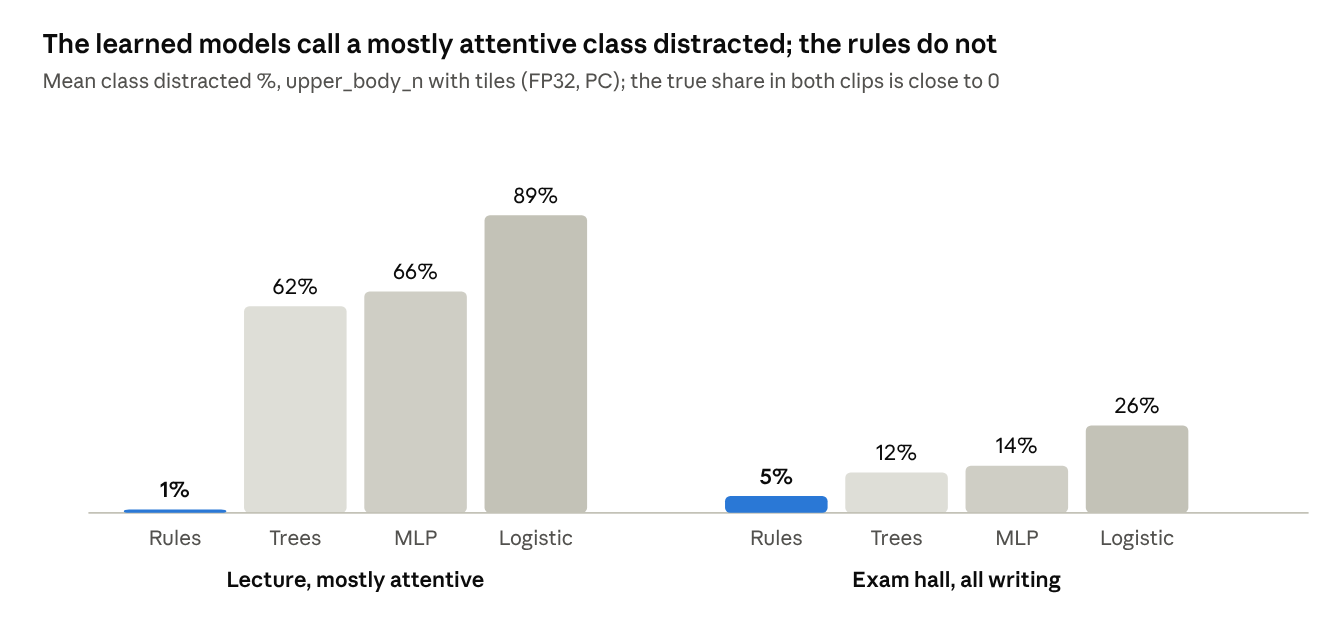
\includegraphics[width=0.9\textwidth]{figures/clips_rules_vs_learned.png}
\caption{Tỷ lệ mất tập trung trung bình của lớp trên video buổi giảng và phòng thi: luật so với các bộ phân loại học máy (upper\_body\_n có chia ô, FP32)}\label{fig:mean-class-distracted-share-on-the-lectu}
\end{figure}

Trong video buổi giảng, học sinh ngồi thẳng nhìn lên bảng bị gán là mất tập trung, còn học sinh cúi đầu đọc bài lại được gán là tập trung (độ cao đầu trung vị so với vai là 0.45 so với 0.32). Nguyên nhân là một khoảng trống trong nhãn của SCB: các lớp tập trung của nó là đọc, viết và giơ tay, đều là cúi đầu hoặc giơ tay, trong khi các lớp mất tập trung gồm quay đầu và thảo luận, đều là ngẩng đầu. SCB không có nhãn ``nghe giảng'' hay ``nhìn lên bảng'', trạng thái chú ý phổ biến nhất trong một buổi giảng, nên mô hình huấn luyện trên SCB học được rằng ngẩng đầu nghĩa là mất tập trung. Loại bỏ các đặc trưng độ cao đầu không khắc phục được điều này trong một thử nghiệm, và các mô hình học máy cũng phụ thuộc mạnh vào chất lượng tư thế: với n và không chia ô, cây quyết định cho 36\% trên video phòng thi trên Pi, so với 9-13\% với m.

Trên các mô hình INT8 khi triển khai, bức tranh vẫn vậy: trong video buổi giảng với m có chia ô, luật cho 0.0\%, còn cây quyết định 48\%, hồi quy logistic 74\% và MLP 52\%.

\textbf{So với nhãn do người gán.} 301 thời điểm học sinh từ video buổi giảng và phòng thi được gán nhãn mù (tập trung, mất tập trung hoặc không rõ), được lấy mẫu sao cho mọi trường hợp bất đồng giữa luật và cây quyết định đều có mặt. Chỉ 13 trên 275 thời điểm có thể đánh giá (4.7\%) là mất tập trung, 4.2\% khi tính lại trọng số cho toàn bộ video. Gộp cả hai video:

\begin{table}[htbp]\small
\caption{Quyết định cho từng học sinh so với 301 nhãn mù do người gán (video buổi giảng và phòng thi)}\label{tab:per-student-decisions-against-301-blind-}
\begin{tabularx}{\textwidth}{*{4}{>{\raggedright\arraybackslash}X}}
\toprule
\textbf{Phương pháp} & \textbf{Báo động nhầm trên thời điểm tập trung} & \textbf{Độ đặc hiệu (KTC 95\%)} & \textbf{Thời điểm mất tập trung phát hiện được} \\
\midrule
Luật & 27 / 262 & 90\% (85-93\%) & 5 / 13 \\
Cây tăng cường gradient & 114 / 262 & 56\% (50-62\%) & 3 / 13 \\
MLP 64-32 & 120 / 262 & 54\% (48-60\%) & 2 / 13 \\
Hồi quy logistic & 199 / 262 & 24\% (19-30\%) & 5 / 13 \\
\bottomrule
\end{tabularx}
\end{table}

Khi tính lại trọng số cho toàn bộ video, các luật đánh dấu 1\% thời điểm của buổi giảng và 3\% thời điểm của phòng thi, gần với giá trị thực 4\%, trong khi các mô hình học máy đánh dấu 56-94\% thời điểm của buổi giảng. Mười ba thời điểm mất tập trung là quá ít để ước lượng recall; các buổi dàn dựng đo đại lượng này.

\textbf{Lớp kiểm tra độc lập (clip\_5).} Cấu hình triển khai giữ được tỷ lệ báo động nhầm thấp trên một lớp được ghi hình sau khi mọi ngưỡng đã được cố định. 150 thời điểm được gán nhãn mù: 121 tập trung, 28 mất tập trung và 1 không rõ, tức 6.8\% mất tập trung khi tính lại trọng số cho toàn bộ video. Các thời điểm được lấy mẫu từ phát hiện của m có chia ô, và một thời điểm mà một lần chạy không phát hiện được tính là không bị đánh dấu. Luận văn không hiển thị khung hình nào của clip\_5, vì học sinh trong đó là trẻ vị thành niên.

\begin{table}[htbp]\footnotesize
\caption{Quyết định cho từng học sinh so với 150 nhãn mù do người gán trên lớp kiểm tra độc lập (clip\_5)}\label{tab:per-student-decisions-against-150-blind-}
\begin{tabularx}{\textwidth}{*{6}{>{\raggedright\arraybackslash}X}}
\toprule
\textbf{Mô hình, có chia ô} & \textbf{Phương pháp} & \textbf{Báo động nhầm trên thời điểm tập trung} & \textbf{Độ đặc hiệu (KTC 95\%)} & \textbf{Mất tập trung phát hiện được} & \textbf{Tỷ lệ bị đánh dấu của video (tính lại trọng số)} \\
\midrule
n & Luật & 11 / 121 & 91\% (84-95\%) & 8 / 28 & 4.7\% \\
n & Cây & 35 / 121 & 71\% (62-78\%) & 3 / 28 & 17.7\% \\
n & Logistic & 44 / 121 & 64\% (55-72\%) & 11 / 28 & 33.9\% \\
n & MLP & 42 / 121 & 65\% (56-73\%) & 9 / 28 & 28.4\% \\
m & Luật & 43 / 121 & 64\% (56-72\%) & 21 / 28 & 10.1\% \\
m & Cây & 51 / 121 & 58\% (49-66\%) & 12 / 28 & 11.4\% \\
m & Logistic & 55 / 121 & 55\% (46-63\%) & 10 / 28 & 35.4\% \\
m & MLP & 37 / 121 & 69\% (61-77\%) & 9 / 28 & 20.0\% \\
\bottomrule
\end{tabularx}
\end{table}

\begin{itemize}
\tightlist
\item
  \textbf{Luật trên n:} độ đặc hiệu 91\%, so với 90\% trên bộ nhãn đầu tiên. Các luật đánh dấu 4.7\% video so với 6.8\% theo nhãn, và phát hiện được 8 trên 28 thời điểm mất tập trung.
\item
  \textbf{Mô hình học máy:} một lần nữa báo động nhầm nhiều hơn hẳn, với độ đặc hiệu 55-71\%.
\item
  \textbf{Luật trên m:} phát hiện được nhiều nhất (21 trên 28) nhưng đánh dấu 36\% thời điểm tập trung. Sáu trong 43 báo động nhầm đó thuộc về một học sinh ở hàng đầu.

  \begin{itemize}
  \tightlist
  \item
    Camera nhìn thấy cả gầm bàn của học sinh đó, nên hộp chuyển qua lại giữa phần thân trên và toàn thân. Các mô hình học hộp toàn thân từ COCO, nơi hộp người bao cả chân.
  \item
    Dấu hiệu \texttt{body\_turned} chia bề rộng vai cho chiều cao hộp, nên hộp cao bị hiểu thành thân xoay.
  \end{itemize}
\item
  \textbf{Không chia ô:} n bỏ sót 92 trên 149 thời điểm.
\item
  \textbf{Đếm chỗ ngồi:} khi có chia ô, bộ phân tích tìm thấy 13-17 chỗ ngồi cho 10 học sinh.

  \begin{itemize}
  \tightlist
  \item
    Chỗ ngồi được neo ở cạnh trên của hộp. Ở khoảng cách gần như vậy, đầu của một học sinh hàng đầu cúi xuống viết di chuyển xa hơn bán kính ghép chỗ ngồi và mở ra một chỗ ngồi mới.
  \item
    Hộp toàn thân thêm một chỗ ngồi thứ hai cho cùng một học sinh.
  \item
    Vì vậy, sau 2:30, chỉ số của lớp với luật có chia ô trung bình 11-15\%, so với 6.8\% theo nhãn.
  \end{itemize}
\end{itemize}

\textbf{Buổi dàn dựng hai người (clip\_4).} Tác giả và một đồng nghiệp, đều là người lớn, ngồi cùng một bàn, được quay bằng một điện thoại gắn cao phía trước, và làm theo kịch bản trong 4:45. Ghi hình theo kịch bản cho biết trạng thái thực của từng người ở mỗi giây. Sau 55 s chú ý, kịch bản có bảy sự kiện mất tập trung:

\begin{itemize}
\tightlist
\item
  nhìn sang bên (hai lần)
\item
  dùng điện thoại dưới gầm bàn và điện thoại trên mặt bàn
\item
  nói chuyện với nhau
\item
  quay ra phía sau
\end{itemize}

Ngoài ra có một phút viết bài, khi đó trạng thái phải giữ là tập trung. Kết quả trên mô hình m INT8 (mô hình n trong ngoặc khi khác biệt):

\begin{table}[htbp]\small
\caption{Buổi dàn dựng hai người (clip\_4), mô hình m INT8}\label{tab:staged-two-person-session-clip-4-int8-m-}
\begin{tabularx}{\textwidth}{*{5}{>{\raggedright\arraybackslash}X}}
\toprule
\textbf{Phương pháp} & \textbf{Số giây mất tập trung phát hiện được} & \textbf{Precision} & \textbf{Báo động nhầm, chú ý / viết} & \textbf{Sự kiện bị bỏ sót} \\
\midrule
Luật, dấu hiệu quay đầu ban đầu & 11\% & 100\% & 0\% / 0\% & 6 trên 7 \\
Cây tăng cường gradient & 40\% (17\%) & 100\% & 0\% / 0\% & 2 trên 7 \\
MLP 64-32 & 40\% (11\%) & 100\% & 0\% / 0\% & 3 trên 7 \\
Hồi quy logistic & 34\% (19\%) & 64\% & 44\% / 0\% & 3 trên 7 \\
Luật với thước đo độ lệch đầu (mặc định mới) & 56\% (45\%) & 100\% & 0\% / 0\% & 2 trên 7 \\
\bottomrule
\end{tabularx}
\end{table}

Không phương pháp nào phát hiện được điện thoại, dù trên mặt bàn hay dưới gầm bàn. Đầu, cổ tay và khuỷu tay nằm trong khoảng 0.2 bề rộng vai so với vị trí của chúng khi viết, nên 13 điểm khóa phần thân trên không thể phân biệt hai trường hợp. Số liệu của các mô hình học máy có trước một bản sửa lỗi ghép chỗ ngồi mô tả dưới đây, nên số giây quay ra phía sau của chúng bị đếm thiếu đôi chút.

\textbf{Vì sao các luật bỏ sót việc quay đầu.} Dấu hiệu quay đầu ban đầu đo góc yaw bằng vị trí của mũi giữa hai tai. Khi nhìn nghiêng, tai phía xa biến mất (độ tin cậy khoảng 0.01), và mã nguồn chuyển sang ước lượng tâm đầu từ tai còn lại. Tai đó đã di chuyển cùng với đầu, nên phép ước lượng triệt tiêu phần lớn góc quay:

\begin{table}[htbp]\small
\caption{Góc yaw dựa trên tai và độ lệch mũi ở các thời điểm chú ý và quay đi của clip\_4}\label{tab:ear-based-yaw-and-nose-offset-at-attenti}
\begin{tabularx}{\textwidth}{*{4}{>{\raggedright\arraybackslash}X}}
\toprule
\textbf{Thời điểm} & \textbf{Người} & \textbf{Yaw dựa trên tai} & \textbf{Độ lệch mũi so với trung điểm vai} \\
\midrule
Chú ý & áo xanh / áo xám & −0.15 / +0.07 & −0.07 / +0.05 \\
Nói chuyện với nhau & áo xám & +0.03 & −0.35 \\
Nhìn sang bên & áo xanh & −0.31 (0.16 so với giá trị gốc) & −0.54 \\
\bottomrule
\end{tabularx}
\end{table}

Độ lệch của mũi so với trung điểm hai vai, tính theo đơn vị bề rộng vai, thể hiện mọi lần quay: khoảng ±0.05 khi chú ý và ±0.35-0.54 khi quay đi. Nó được thêm vào làm thước đo góc quay đầu thứ hai, so với độ lệch đã hiệu chỉnh của chính chỗ ngồi đó. Dấu hiệu lấy thước đo nào cho thấy góc quay lớn hơn trong hai thước đo. Giống như yaw, giá trị gốc về độ lệch của mỗi chỗ ngồi được giữ trong phạm vi 0.15 so với giá trị của cả phòng, để một học sinh nhìn đi chỗ khác trong lúc hiệu chỉnh không học ``quay đi'' thành trạng thái chú ý. Cùng buổi dàn dựng đó cũng cho thấy một học sinh quay ra phía sau co lại thành một hộp chỉ gồm đầu và vai, có tâm nhảy khoảng một phần ba chiều cao hộp, nên chỗ ngồi giờ được neo ở cạnh trên của hộp.

\textbf{Kiểm chứng bản sửa.} Các ngưỡng của thước đo độ lệch được chọn bằng clip\_4, nên recall trên clip\_4 mang tính lạc quan. Vì vậy chi phí của nó được đo trên mọi dữ liệu còn lại, bằng một lần quét 16 thiết lập trên các bộ khung xương INT8 đã lưu. Ở hàm dốc được chọn (0.2-0.4, các ngưỡng khác giữ nguyên):

\begin{table}[htbp]\small
\caption{Tác dụng của thước đo độ lệch đầu trên toàn bộ bằng chứng}\label{tab:effect-of-the-head-offset-measure-across}
\begin{tabularx}{\textwidth}{*{3}{>{\raggedright\arraybackslash}X}}
\toprule
\textbf{} & \textbf{n, trước → sau} & \textbf{m, trước → sau} \\
\midrule
Số giây mất tập trung phát hiện được trên clip\_4 & 11\% → 45\% & 11\% → 56\% \\
Nhãn người gán: báo động nhầm trên thời điểm tập trung & 4\% → 5\% & 6\% → 7\% \\
Tỷ lệ của lớp, buổi giảng (giá trị thực gần 0) & 4.7\% → 4.7\% & 0.0\% → 0.0\% \\
Tỷ lệ của lớp, phòng thi & 3.6\% → 8.4\% & 11.7\% → 14.6\% \\
\bottomrule
\end{tabularx}
\end{table}

Chi phí duy nhất là 3-5 điểm trên video phòng thi. Một phần trong đó có thể là thật, vì nhãn người gán cho thấy học viên phòng thi có nhìn quanh. Chỉ nới lỏng các ngưỡng yaw thì chỉ đạt 25\% trên clip\_4. Thước đo này giờ là mặc định, và buổi học 9 người được giữ làm bài kiểm tra độc lập.

Thước đo này chỉ giúp các luật. Các bộ phân loại học máy quyết định dựa trên các đặc trưng chúng đã được huấn luyện, vốn không gồm thước đo này. Nó cũng không thể học từ SCB: nó cần giá trị gốc theo từng học sinh, và trên các ảnh đơn lẻ với khuôn mặt nhỏ của SCB, nó không phân biệt được đầu quay đi với đọc bài (AUC 0.53).

\begin{figure}[htbp]
\centering
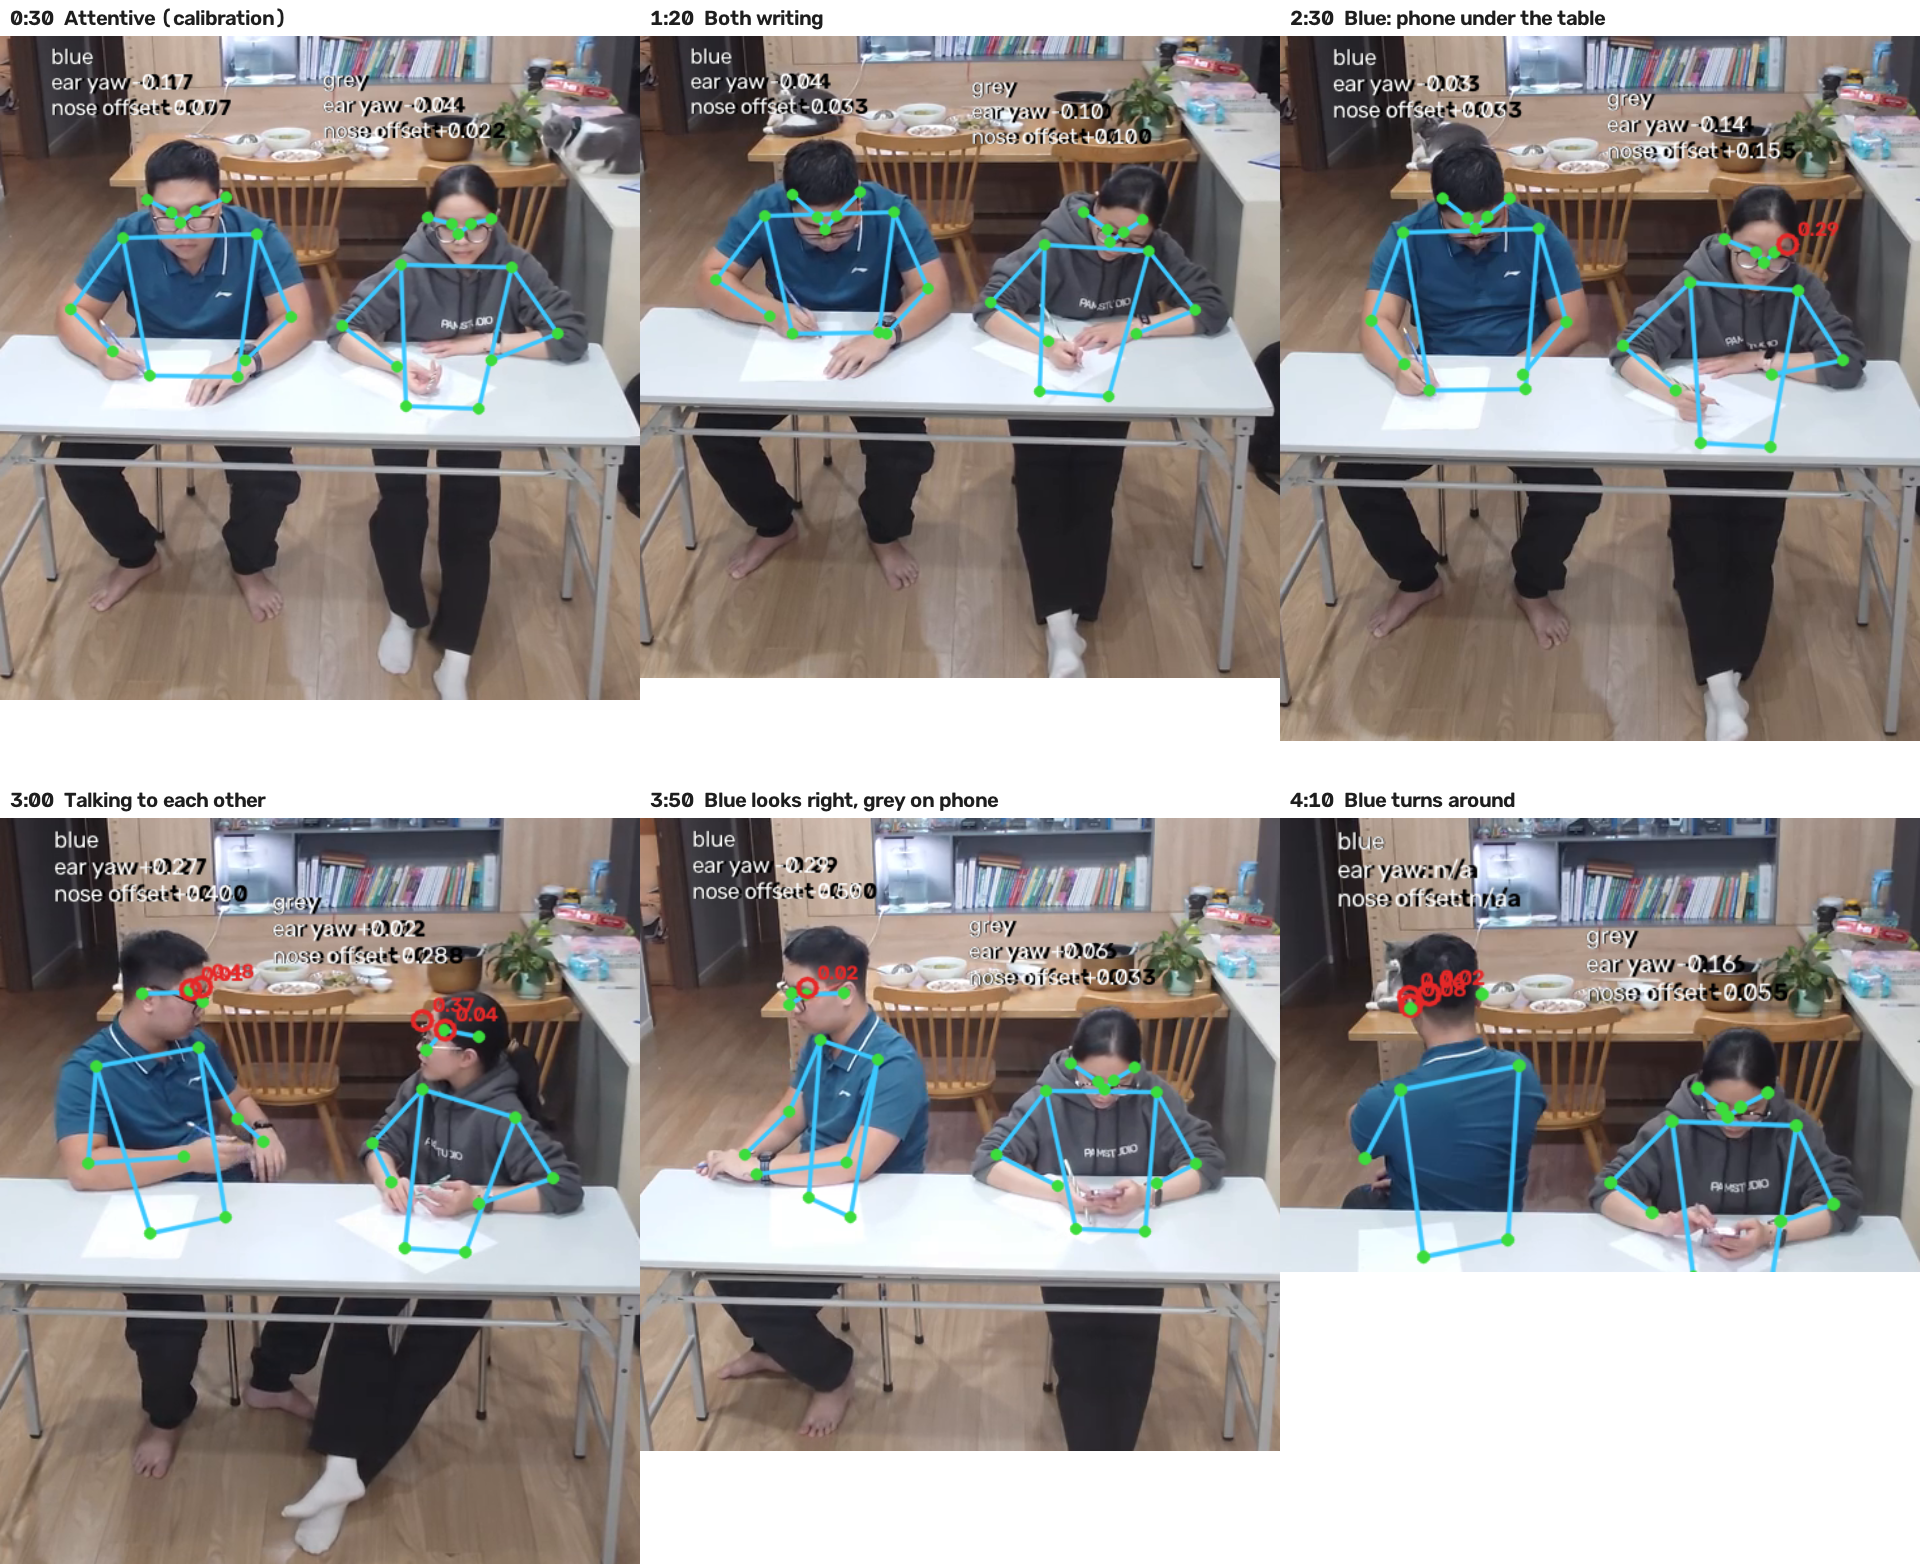
\includegraphics[width=1.0\textwidth]{figures/clip4_overview.png}
\caption{Những gì mô hình tư thế thấy trên clip\_4, với hai thước đo góc quay đầu của từng người}\label{fig:what-the-pose-model-sees-on-clip-4-with-}
\end{figure}

Khi nhìn nghiêng, độ tin cậy của tai phía xa giảm còn khoảng 0.01, nên yaw dựa trên tai đọc gần bằng 0 trong khi mũi nằm lệch hẳn về một phía so với vai. Thước đo độ lệch đầu bắt được những lần quay này.

Vì vậy, độ chính xác trên benchmark của một bộ phân loại huấn luyện trên một bộ dữ liệu hành động công khai không chuyển giao sang việc đo sự chú ý; hiệu chỉnh theo từng học sinh cho kết quả tốt hơn. Để một mô hình học máy dùng được, cần nhãn huấn luyện có cả những học sinh ngẩng đầu chú ý từ chính các lớp học mục tiêu, điều mà các nhãn người gán đang thực hiện và buổi dàn dựng bắt đầu cung cấp.

\section{Hiệu năng trên thiết bị biên}

Trong cấu hình triển khai, n có chia ô chạy thời gian thực, hệ thống chạy 15 phút ở 30 FPS với độ trễ 45 ms, công suất đo được 4.3 W trên bo mạch Pi cộng 2.5 W cho Hailo-8 (số liệu nhà sản xuất), nhiệt độ SoC cao nhất 60 °C và không bị giảm xung. Pipeline bị giới hạn bởi Hailo-8, không phải CPU. Mọi số liệu dưới đây được đo trên Pi 5 với bộ tản nhiệt chủ động chính hãng Raspberry Pi gắn vào cổng quạt, ngày 10/11/2026.

\textbf{Riêng Hailo-8} (\texttt{hailortcli\ benchmark}, HEF INT8):

\begin{table}[htbp]\small
\caption{Thông lượng và độ trễ của Hailo-8 theo mô hình (hailortcli benchmark)}\label{tab:hailo-8-throughput-and-latency-per-model}
\begin{tabularx}{\textwidth}{*{3}{>{\raggedright\arraybackslash}X}}
\toprule
\textbf{Mô hình} & \textbf{FPS} & \textbf{Độ trễ phần cứng (ms)} \\
\midrule
n & 131.5 & 5.7 \\
s & 69.5 & 11.9 \\
m & 31.5 & 26.7 \\
\bottomrule
\end{tabularx}
\end{table}

\textbf{Đầu cuối} (video buổi giảng, 1280×720, engine GStreamer, bật đánh giá mức độ tập trung, chạy nhanh nhất có thể):

\begin{table}[htbp]\footnotesize
\caption{Hiệu năng đầu cuối trên Raspberry Pi 5 (video buổi giảng, 1280×720)}\label{tab:end-to-end-performance-on-the-raspberry-}
\begin{tabularx}{\textwidth}{*{7}{>{\raggedright\arraybackslash}X}}
\toprule
\textbf{Mô hình} & \textbf{Chia ô} & \textbf{FPS} & \textbf{CPU, toàn bộ Pi} & \textbf{Bộ nhớ của hcpose (MB)} & \textbf{Nhiệt độ SoC tối đa (°C)} & \textbf{Công suất bo mạch Pi (W)} \\
\midrule
n & tắt & 119.1 & 79\% & 332 & 61.1 & 5.42 \\
n & bật & 32.8 & 46\% & 286 & 60.6 & 4.84 \\
s & tắt & 69.3 & 47\% & 329 & 60.1 & 4.77 \\
s & bật & 17.4 & 26\% & 294 & 59.5 & 3.87 \\
m & tắt & 31.5 & 23\% & 339 & 58.4 & 3.19 \\
m & bật & 7.9 & 14\% & 307 & 57.3 & 2.82 \\
\bottomrule
\end{tabularx}
\end{table}

FPS đầu cuối khớp với số liệu khi chỉ chạy Hailo, và bốn lượt mỗi khung hình chia chúng đúng cho bốn. Chi phí chính của CPU là phần phân tích mức độ tập trung, khoảng 2.8 lõi ở 119 FPS. Công suất bo mạch thấp hơn ở các thiết lập chậm hơn vì Pi phải chờ bộ tăng tốc.

\textbf{Độ trễ.} Khung hình được đưa vào ở tốc độ 25 FPS của video, giống như camera đưa ra, và được đo thời gian từ thời điểm đó đến sink bằng bộ đo interlatency của GstShark \cite{b20}: trung vị 20 ms cho n (phân vị 95 là 23), 45 ms cho n có chia ô (53), và 40 ms cho m (47). m có chia ô không theo kịp camera 25 FPS (7.9 FPS): khung hình bị xếp hàng và độ trễ ổn định ở 2.5 s, nên triển khai trực tiếp m có chia ô cần một hàng đợi có bỏ khung hình (leaky queue) hoặc giảm tốc độ camera.

\textbf{Đặc tính nhiệt} qua hai lần chạy 15 phút:

\begin{table}[htbp]\footnotesize
\caption{Đặc tính nhiệt qua các lần chạy 15 phút}\label{tab:thermal-behaviour-over-15-minute-runs}
\begin{tabularx}{\textwidth}{*{6}{>{\raggedright\arraybackslash}X}}
\toprule
\textbf{Lần chạy} & \textbf{FPS} & \textbf{Nhiệt độ SoC sau 5 / 10 / 15 phút (°C)} & \textbf{Tối đa (°C)} & \textbf{Giảm xung} & \textbf{Công suất bo mạch Pi (W)} \\
\midrule
n có chia ô, thời gian thực (triển khai) & 30.0 & 56.8 / 57.9 / 56.8 & 60.1 & không & 4.26 \\
m có chia ô, nhanh nhất có thể & 7.9 & 53.5 / 55.6 / 54.6 & 56.2 & không & 2.70 \\
\bottomrule
\end{tabularx}
\end{table}

Khi rảnh, Pi tiêu thụ 2.33 W ở 50 °C.

\textbf{Công suất.} Công suất bo mạch là tổng điện áp × dòng điện trên các đường nguồn PMIC của Pi 5 (\texttt{vcgencmd\ pmic\_read\_adc}). Con số này không gồm AI HAT và các thiết bị USB, nên Hailo-8 được cộng thêm từ số liệu nhà sản xuất:

\begin{table}[htbp]\small
\caption{Số liệu công suất của nhà sản xuất dùng để bổ sung cho công suất bo mạch đo được}\label{tab:vendor-power-figures-used-to-complete-th}
\begin{tabularx}{\textwidth}{*{3}{>{\raggedright\arraybackslash}X}}
\toprule
\textbf{Thành phần} & \textbf{Số liệu} & \textbf{Nguồn} \\
\midrule
Raspberry Pi 5, dòng hoạt động điển hình của bo mạch trần & 800 mA ở 5 V ≈ 4 W & \href{https://www.raspberrypi.com/documentation/computers/raspberry-pi.html\#power-supply}{Tài liệu Raspberry Pi} \cite{b21} \\
Raspberry Pi 5, nguồn khuyến nghị & 5 V, 5 A (27 W) & như trên \\
Hailo-8, công suất điển hình & 2.5 W & \href{https://hailo.ai/products/ai-accelerators/hailo-8-ai-accelerator/}{Hailo} \cite{b5} \\
Mô-đun Hailo-8 M.2, tối đa & 8.65 W & \href{https://core-electronics.com.au/hailo-8-m2-ai-accelerator-module-26-tops.html}{Trang sản phẩm Core Electronics} \cite{b22} \\
AI HAT+, nhiệt độ môi trường hoạt động & 0-50 °C & \href{https://cdn.sparkfun.com/assets/c/9/b/7/3/Raspberry_Pi_AI_HAT__product_brief.pdf}{Tài liệu tóm tắt AI HAT+} \cite{b23} \\
\bottomrule
\end{tabularx}
\end{table}

Vì vậy cấu hình triển khai tiêu thụ khoảng 4.3 W (đo được) + 2.5 W (điển hình, theo nhà sản xuất) ≈ 6.8 W, nằm trong khả năng của một nguồn USB-C 27 W. Số liệu đo trên bo mạch khớp với mức điển hình 4 W của nhà sản xuất. 26 TOPS ở 2.5 W tương đương khoảng 10 TOPS/W (tác giả tự tính từ số liệu của Hailo).

\section{Quyền riêng tư từ thiết kế}

Theo mặc định, hệ thống không bao giờ lưu hay truyền đi hình ảnh: mỗi khung hình chỉ tồn tại trong bộ nhớ trong một lần suy luận, và đầu ra mặc định duy nhất là một tỷ lệ cấp lớp hiển thị trên màn hình của giáo viên.

\begin{figure}[htbp]
\centering
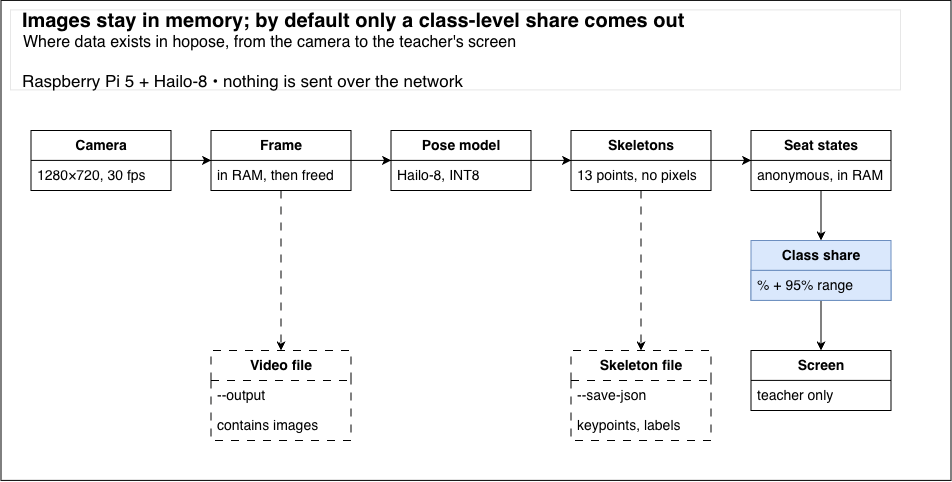
\includegraphics[width=0.9\textwidth]{figures/dataflow.png}
\caption{Luồng dữ liệu trong hcpose với thiết lập mặc định; các đầu ra tùy chọn vẽ nét đứt}\label{fig:data-flow-in-hcpose-with-default-setting}
\end{figure}

\begin{itemize}
\tightlist
\item
  \textbf{Khung hình} được giải mã vào RAM, chuyển tới Hailo-8 rồi giải phóng. Không gì được ghi xuống đĩa trừ khi đặt \texttt{-\/-output}, tùy chọn dành cho phát triển và đánh giá, không dành cho lớp học.
\item
  \textbf{Bộ khung xương} (13 điểm khóa và một hộp cho mỗi người) không chứa điểm ảnh. Tự chúng không định danh được ai, nhưng khi gắn với một chỗ ngồi và một thời điểm trong một lớp đã biết, chúng có thể chỉ ra một học sinh, nên chúng được coi là dữ liệu cá nhân và chỉ giữ trong bộ nhớ.
\item
  \textbf{Trạng thái chỗ ngồi} dùng số chỗ ngồi ẩn danh chỉ tồn tại trong một phiên. Không có nhận diện khuôn mặt, không có danh sách tên và không có liên kết giữa các phiên, ngoại trừ một tệp hiệu chỉnh tùy chọn (\texttt{-\/-calibration}) lưu tư thế chú ý và vị trí của mỗi chỗ ngồi, không lưu danh tính.
\item
  \textbf{Tỷ lệ của lớp} kèm khoảng của nó là con số duy nhất được thiết kế để ra khỏi chương trình. Nó mô tả lớp học, không mô tả một học sinh, và không phải là dữ liệu cá nhân.
\item
  \textbf{Màn hình} hiển thị ảnh camera kèm nhãn trong quá trình phát triển. Khi dùng trong lớp, \texttt{-\/-display\ class} giới hạn phần hiển thị chỉ còn con số của lớp, và \texttt{-\/-headless} không mở cửa sổ nào.
\item
  \textbf{Mạng:} hcpose không mở kết nối mạng nào; thiết bị có thể chạy hoàn toàn ngoại tuyến.
\end{itemize}

Nội dung một bản ghi được lưu khi dùng \texttt{-\/-save-json}: mỗi khung hình một dòng, lấy từ clip\_4 tại 3:50, rút gọn còn một người và ba trong 13 điểm khóa. Bản ghi có tọa độ, điểm số và trạng thái, nhưng không có điểm ảnh và không có danh tính. Số chỗ ngồi chỉ tồn tại trong phiên.

\begin{codeblock}
{"type": "frame", "t": 229.97, "w": 1280, "h": 720,
 "class": {"visible": 2, "counted": 2, "focused": 1, "distracted": 1,
           "class_pct_distracted": 33.3, "class_ci": [6.1, 79.2], "class_size": 3},
 "persons": [{"score": 0.75, "box": [663.9, 296.1, 863.6, 709.2],
              "keypoints": [[771.9, 356.1, 0.98], [776.5, 348.7, 0.91], [761.6, 349.6, 0.95], "…"],
              "engagement": {"seat": 2, "state": "focused", "score": 0.0, "reason": null, "calibrated": true}}]}
\end{codeblock}

So với một dịch vụ đám mây, không có gì phải tải lên, được bên thứ ba lưu trữ hay chuyển ra nước ngoài, nhờ đó loại bỏ các nghĩa vụ về chuyển dữ liệu xuyên biên giới và phần lớn rủi ro rò rỉ.

\section{Sự phù hợp với pháp luật Việt Nam}

Từ ngày 1/1/2026, dữ liệu cá nhân tại Việt Nam được điều chỉnh bởi Luật Bảo vệ dữ liệu cá nhân (Luật số 91/2025/QH15) \cite{b12} và Nghị định hướng dẫn thi hành 356/2025/NĐ-CP, thay thế Nghị định 13/2023/NĐ-CP. Việc giữ video trên thiết bị và chỉ báo cáo một tỷ lệ cấp lớp làm giảm, nhưng không xóa bỏ, các nghĩa vụ của một trường học khi sử dụng hệ thống. Mục này là phân tích phục vụ luận văn, không phải tư vấn pháp lý.

\begingroup\small
\begin{xltabular}{\textwidth}{*{3}{>{\raggedright\arraybackslash}X}}
\caption{Các quy định của Luật 91/2025/QH15 và Nghị định 356/2025/NĐ-CP và hệ quả đối với hệ thống}\label{tab:provisions-of-law-91-2025-qh15-and-decre}\\
\toprule
\textbf{Quy định} & \textbf{Nội dung} & \textbf{Hệ quả đối với hệ thống} \\
\midrule
\endfirsthead
\multicolumn{3}{l}{\emph{(tiếp theo)}}\\
\toprule
\textbf{Quy định} & \textbf{Nội dung} & \textbf{Hệ quả đối với hệ thống} \\
\midrule
\endhead
\bottomrule
\endlastfoot
Dữ liệu cá nhân (Luật, Điều 2.1) & dữ liệu ``xác định hoặc giúp xác định một con người cụ thể'' & Khung hình camera là dữ liệu cá nhân. Điểm khóa gắn với một chỗ ngồi và một thời điểm trong một lớp đã biết có thể giúp xác định một học sinh, nên bộ khung xương và nhãn theo từng học sinh cũng được coi là dữ liệu cá nhân; tỷ lệ cấp lớp thì không. \\
Dữ liệu nhạy cảm (Luật, Điều 2.3; Nghị định 356, Điều 4) & dữ liệu gắn với quyền riêng tư, theo danh mục của Chính phủ, bao gồm dữ liệu sinh trắc học & hcpose không nhận diện khuôn mặt và không lưu danh tính. Việc điểm khóa cơ thể dùng để phân tích hành vi có được coi là sinh trắc học hay không chưa được xác định rõ, nên thiết kế coi dữ liệu theo từng học sinh như dữ liệu nhạy cảm: mặc định chỉ giữ trong bộ nhớ, không bao giờ truyền đi. \\
Giới hạn mục đích (Luật, Điều 3.2) & xử lý ``cho mục đích cụ thể, rõ ràng'' & Một mục đích được nêu rõ: chỉ số chú ý tổng hợp cho giáo viên. Không có báo cáo, xếp hạng hay chấm điểm theo từng học sinh. \\
Sự đồng ý (Luật; Nghị định 356, Điều 9) & đồng ý theo từng mục đích; không có đồng ý mặc định hay gộp & Nhà trường thông báo cho học sinh và phụ huynh và có được sự đồng ý cho camera và mục đích này trước khi triển khai. \\
Trẻ em (Luật, Điều 24.2) & người đại diện theo pháp luật thực hiện thay trẻ em; trẻ từ đủ 7 tuổi trở lên cũng phải đồng ý khi đời sống riêng tư bị tiết lộ & Phần lớn học sinh là người chưa thành niên: cần sự đồng ý của cha mẹ, và học sinh lớn hơn cũng nên được thông báo và hỏi ý kiến. \\
Ghi hình ở nơi công cộng (Luật, Điều 32) & chỉ được phép không cần đồng ý với các hoạt động công cộng được liệt kê, có thông báo & Một tiết học không thuộc các trường hợp được liệt kê, nên áp dụng con đường xin đồng ý nêu trên. \\
Đánh giá tác động (Luật; Nghị định 356) & đánh giá tác động xử lý dữ liệu, cập nhật khi việc xử lý thay đổi & Trường triển khai hệ thống cần lập DPIA. Thời gian ân hạn cho doanh nghiệp nhỏ không áp dụng cho việc trực tiếp xử lý dữ liệu nhạy cảm. \\
Thông báo vi phạm & trong vòng 72 giờ & Mặc định không lưu gì nên có rất ít dữ liệu có thể bị rò rỉ; mọi tệp được lưu đều thuộc phạm vi quy định này. \\
\end{xltabular}
\endgroup

\textbf{Đóng góp của thiết kế.} Tối thiểu hóa dữ liệu và giới hạn lưu trữ được tích hợp sẵn: khung hình chỉ tồn tại trong RAM trong thời gian một lần suy luận, không có gì rời khỏi thiết bị, và đầu ra mặc định là một con số cấp lớp. Những việc vẫn thuộc trách nhiệm của nhà trường: thông báo, xin đồng ý, lập DPIA, và giữ tắt các đầu ra nghiên cứu tùy chọn (video có chú thích, tệp khung xương) khi sử dụng thực tế.

Nguồn: \cite{b12,b24,b25,b26,b27}. Số điều khoản theo bản dịch tiếng Anh; cần đối chiếu với văn bản tiếng Việt chính thức trước khi trích dẫn.

\section{Hạn chế}

Khoảng trống lớn nhất là dữ liệu chuẩn: đến nay chưa có kết quả nào đo độ chính xác theo từng học sinh trên một buổi giảng thực, mà chỉ trên các hành động của SCB hoặc thông qua bối cảnh của các video phần lớn học sinh chăm chú.

\begin{itemize}
\tightlist
\item
  \textbf{Nhãn thay thế.} SCB gán nhãn hành động (đọc, quay đầu, thảo luận), không gán nhãn sự chú ý, và chủ yếu lấy từ lớp học phổ thông Trung Quốc. Khoảng 2.000 học sinh SCB mang cả nhãn tập trung lẫn mất tập trung trên các ảnh trùng, phần lớn là ``cúi đầu'' so với ``đọc hoặc viết'', nên ngay cả người gán nhãn cũng không phân biệt được các trường hợp này.
\item
  \textbf{Bằng chứng từ video dựa vào bối cảnh.} Ba video không có nhãn; nhận định ``tỷ lệ thực gần 0'' dựa trên việc lớp học đang làm gì. Chúng cho thấy báo động nhầm, chứ không cho thấy mất tập trung bị bỏ sót. Nhãn người gán và buổi dàn dựng giải quyết vấn đề này.
\item
  \textbf{Ít phòng học, video của bên thứ ba.} Ba video của bên thứ ba từ ba phòng học, một trong số đó có camera đặt ngoài vị trí lắp đặt dự kiến, cùng một lớp nhỏ được ghi hình cho luận văn này. Kết quả có thể không đúng với các cách bố trí, điều kiện ánh sáng hay lứa tuổi khác.
\item
  \textbf{Độ cao camera.} Với camera ngang mặt bàn, một cái đầu cúi xuống viết sẽ che khuôn mặt và bị hiểu là ``quay đi'': các luật cho 44\% mất tập trung trong một phòng tự học nơi mọi người đều đang viết. Thiết kế giả định camera gắn cao phía trước; giảm trọng số \texttt{face\_hidden} (0.3) làm lỗi giảm một nửa với camera thấp.
\item
  \textbf{Thời gian hiệu chỉnh.} Mỗi chỗ ngồi cần 120 s quan sát dùng được. Trong một video dày đặc dài 6 phút, chỉ 20 trên 52 chỗ ngồi hoàn tất hiệu chỉnh, nên các phiên ngắn chủ yếu chạy với giá trị gốc ở cấp phòng.
\item
  \textbf{Lớp nhỏ, khoảng rộng.} Với 20-30 học sinh được đếm, khoảng 95\% rộng 25-37 điểm trừ khi biết sĩ số. Đây là tính chất của cỡ mẫu, không phải khiếm khuyết, nhưng nó giới hạn độ mịn khi đọc chỉ số.
\item
  \textbf{Trọng số luật đặt thủ công.} Trọng số của các luật được đặt theo thiết kế, không được khớp từ dữ liệu, và cố ý không tinh chỉnh trên các video dùng để đánh giá chúng; một thay đổi đã ghi nhận, trọng số cho camera thấp, là một tùy chọn chứ không phải mặc định.
\item
  \textbf{Độ chính xác số học không đồng nhất giữa các bằng chứng.} Hai biểu đồ và điểm số theo nhãn người gán dùng mô hình n ở FP32 trên PC; các lần chạy INT8 trên Pi tái hiện các con số cấp lớp với sai khác vài điểm. m có chia ô cũng không theo kịp camera trực tiếp 25-30 FPS nếu không bỏ khung hình.
\item
  \textbf{Buổi dàn dựng.} Các tình nguyện viên người lớn diễn hành vi theo kịch bản trong một phòng nhỏ dễ thấy hơn và cường điệu hơn so với mất tập trung thực, nên recall của buổi này là một cận trên.
\item
  \textbf{Camera ở gần và hộp toàn thân.} Trong một phòng nhỏ quay ở khoảng cách gần, số chỗ ngồi bị nhân lên (13-17 cho 10 học sinh trong clip\_5), và hộp toàn thân của một học sinh thấy được chân bị hiểu là thân xoay. Cả hai đều xuất phát từ hình học gắn với hộp: điểm neo chỗ ngồi ở cạnh trên của hộp và chiều cao hộp trong \texttt{body\_turned}. Neo và tỷ lệ dựa trên điểm khóa sẽ tránh được các vấn đề này; chúng không được thay đổi sau clip\_5, để giữ clip\_5 là một bài kiểm tra độc lập.
\end{itemize}
